\section{Solution}

\subsection{Mobile Terminal Part}

\subsubsection{Flow Chart}

   First the motion of one person is detected by the sensor and become raw data.
   Then the raw data is filtered into acceleration data. 

   The filter mainly did two things.
   One is to abandon the useless data such as temperature and the other is to
   map the acceleration data into float point value between 0 to 5. 

   After that, the acceleration data will be processed through one of the
   following function, which are the \textbf{Matcher} and the \textbf{Scaler}. 

   After the the process of \textbf{Matcher} or \textbf{Scaler} function, one
   sound track is created and finally the multiple sound tracks are mixed into
   the final audio. 

\subsubsection{Index Script}

The Unity Engine first recognize the index script and hand over its control to
it.  
Thus, we use the index script to get access to the 
\textbf{gyroscope}, \textbf{speaker} of the mobile phone, 
 ask for \textbf{memory}, create \textbf{main loop} (the loop in which the
 program will be in after initial setup), and call for 
\textbf{Matcher} and \textbf{Scaler} functions. 
The flow chart of the index script is shown in Figure~\ref{indexScript}.


\begin{figure}[H]

\begin{minipage}[b]{0.5\linewidth}
\centering
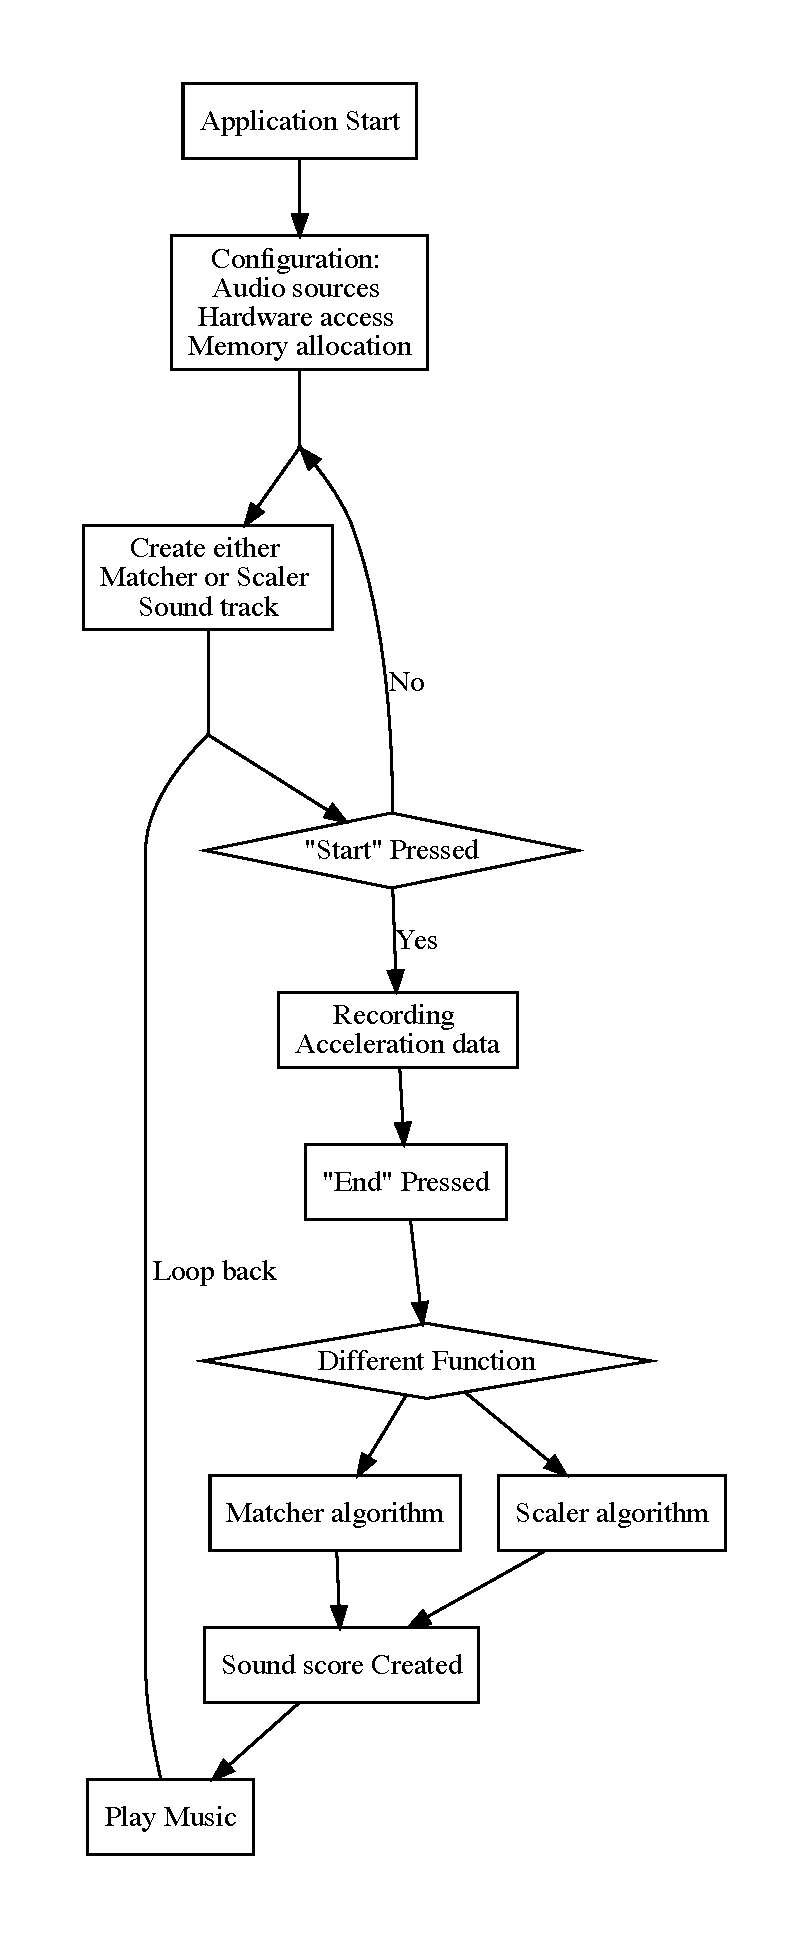
\includegraphics[height=0.95\textheight]{figWR/a}
\caption{Flow Chart of the Index Script}
\label{indexScript}
\end{minipage}%%
%
\begin{minipage}[b]{0.5\linewidth}
\centering
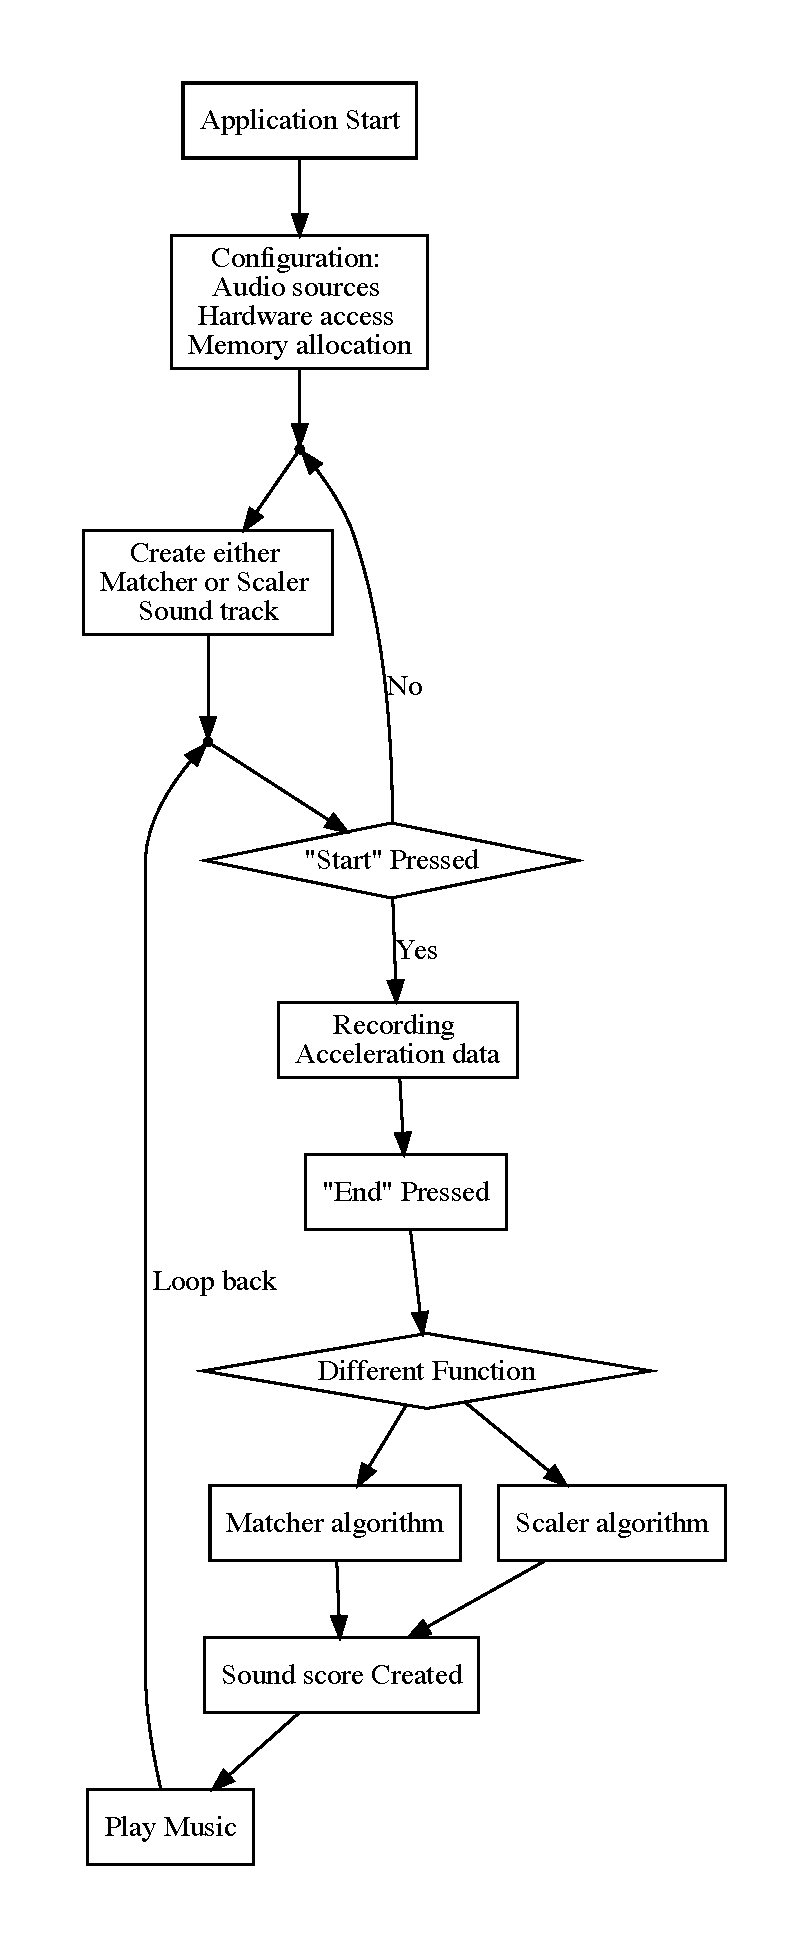
\includegraphics[width=1\linewidth]{figWR/ma}
\caption{Flow Chart of Matcher}
\label{FlowMatcher}
\vspace{4ex}
\centering
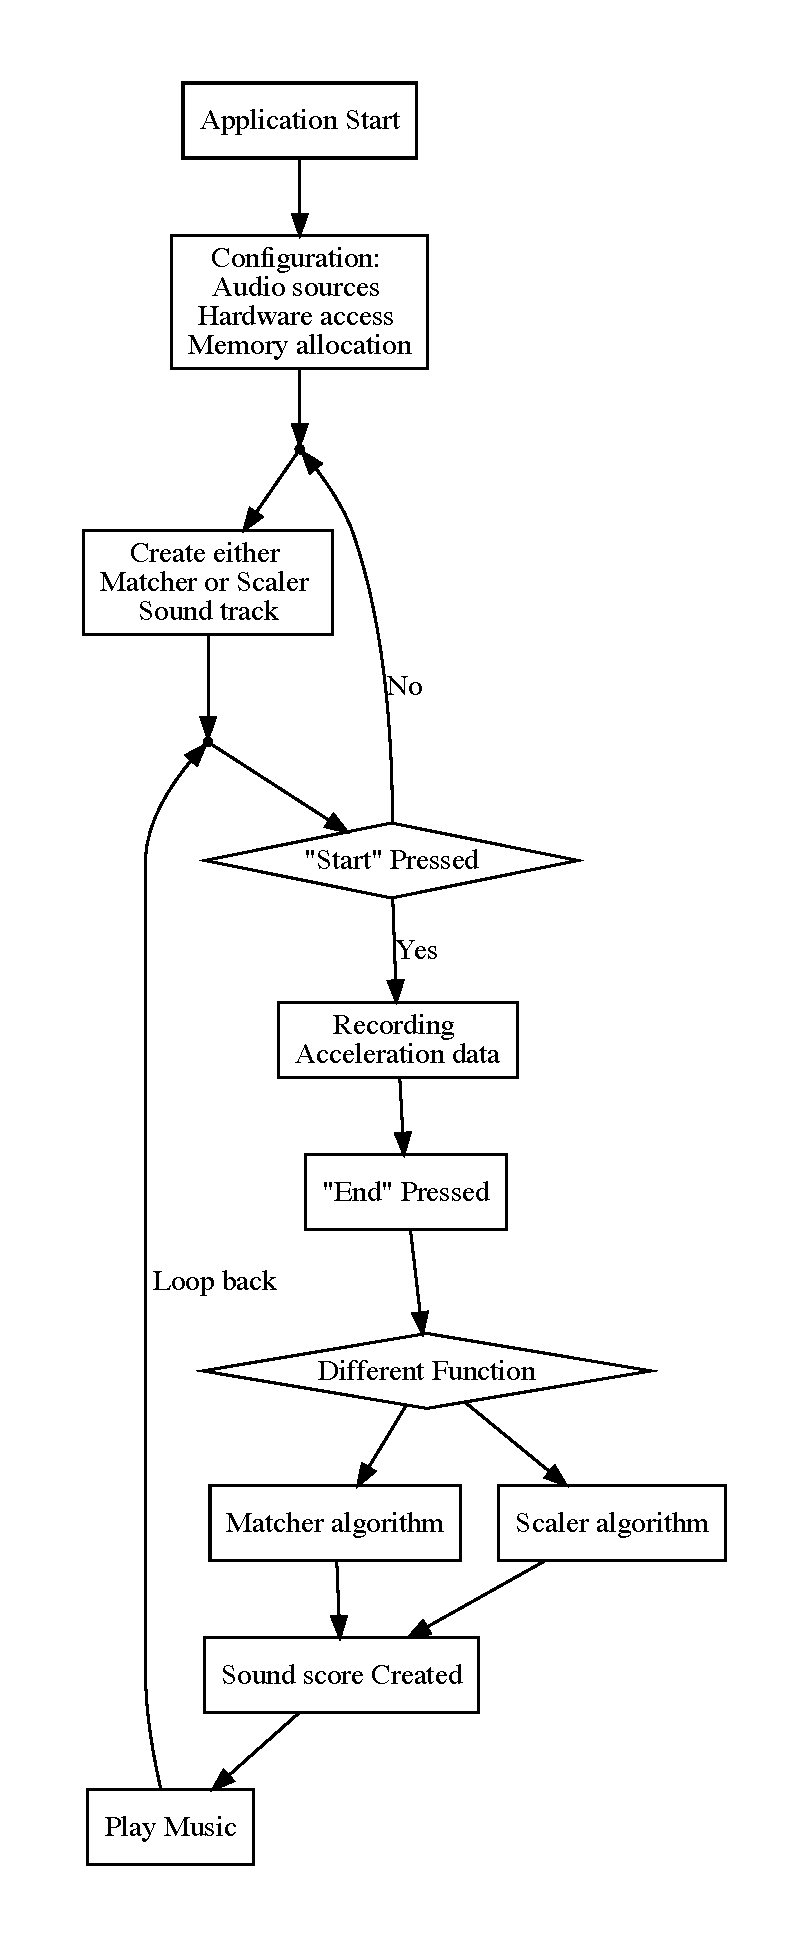
\includegraphics[width=1\linewidth]{figWR/sc}
\caption{Flow Chart of Scaler}
\label{FlowMatcher}
\vspace{4ex}
\end{minipage}%%
\end{figure}

\subsubsection{Scaler algorithm}

   For the \textbf{Scaler} part, also suppose we have the acceleration data.
   Then we separate them into 10 time intervals equally.
   And we find the max value in each interval.
   Then the ruler is created based on the max value and the min value of the
   acceleration data.
   The ruler create 7 blanks vertically for there is 7 tones in one music
   period, which are ``do re mi fa so la si''.
   Fill in the blank and finally a music score is created and it produces one
   sound track.

   The visual of the \textbf{Scaler} process is shown by step in
   Figure~\ref{scalerStep0} to Figure~\ref{scalerStep2}.  

\begin{figure}[H]
\centering
\newcommand{\widthOfScalerStepFigure}{5cm}
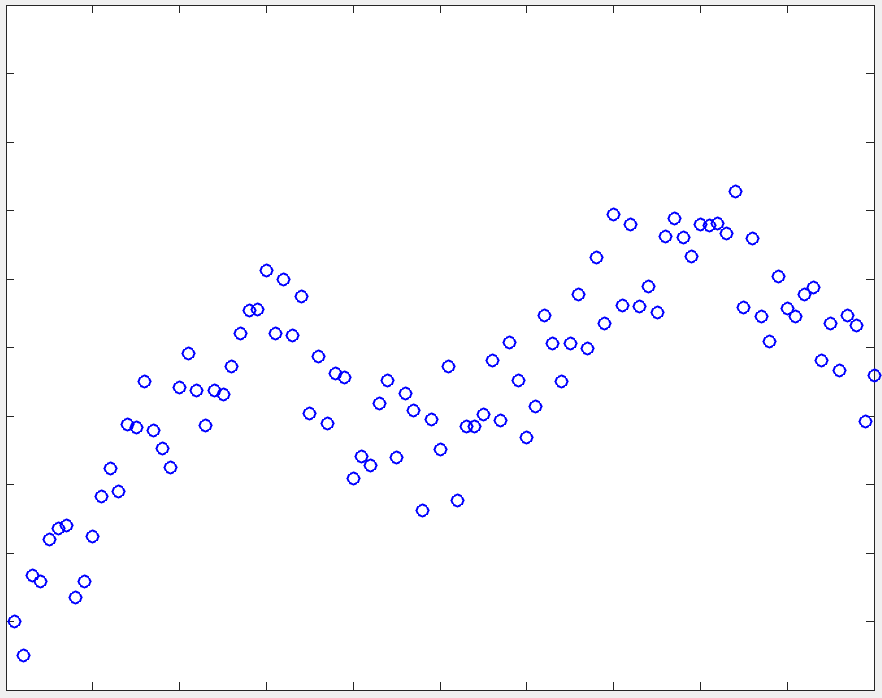
\includegraphics[width=\widthOfScalerStepFigure]{figWR/scaler0}
\caption{Scaler Process, original data}
\label{scalerStep0}
\end{figure}

\begin{figure}[H]
\centering
\newcommand{\widthOfScalerStepFigure}{5cm}
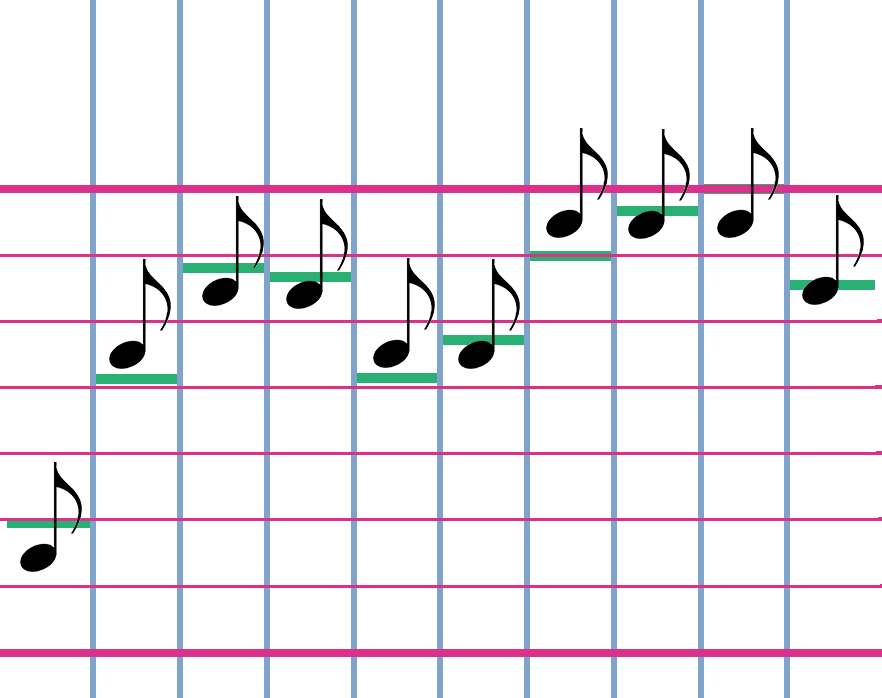
\includegraphics[width=\widthOfScalerStepFigure]{figWR/scaler1}
\caption{Scaler Process, split and create ruler}
\label{scalerStep1}
\end{figure}

\begin{figure}[H]
\centering
\newcommand{\widthOfScalerStepFigure}{5cm}
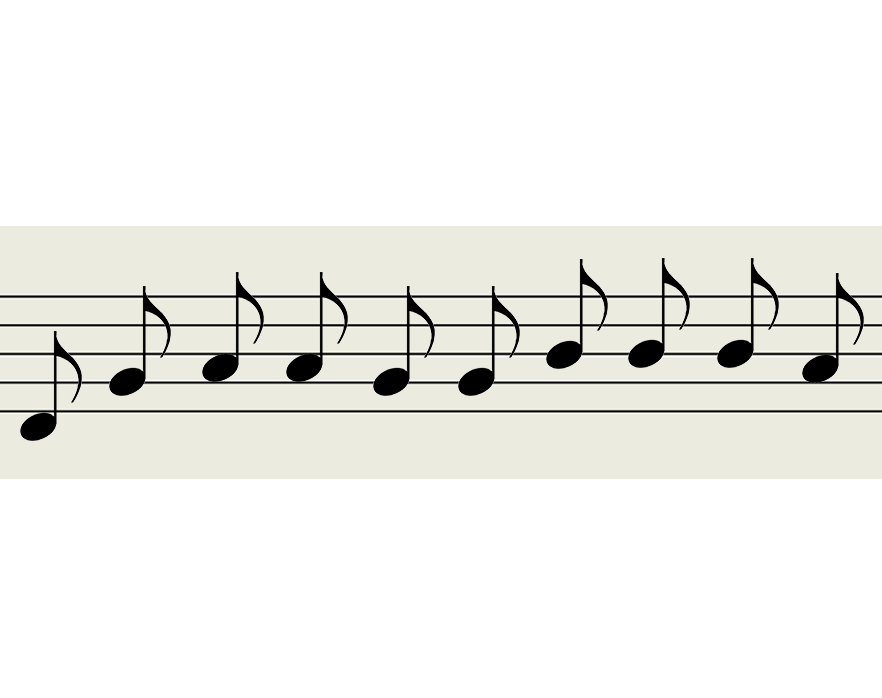
\includegraphics[width=\widthOfScalerStepFigure]{figWR/scaler2}
\caption{Scaler Process, final music score}
\label{scalerStep2}
\end{figure}


\subsubsection{Matcher algorithm}

   For the \textbf{Matcher} part, suppose we have the acceleration data,
   then we compared it with three pre-configured answers,
   calculate the difference between answers and real data.
   The one that has the least sum of absolute value is the audio clip we select.
   Then the corresponding sound track is created.

   The visual of the \textbf{Matcher} process is shown in
   Figure~\ref{matcherStep0} and Figure~\ref{matcherStep1}. 


\newcommand{\widthOfMatcherFigure}{10cm}
\begin{figure}[H]
\centering
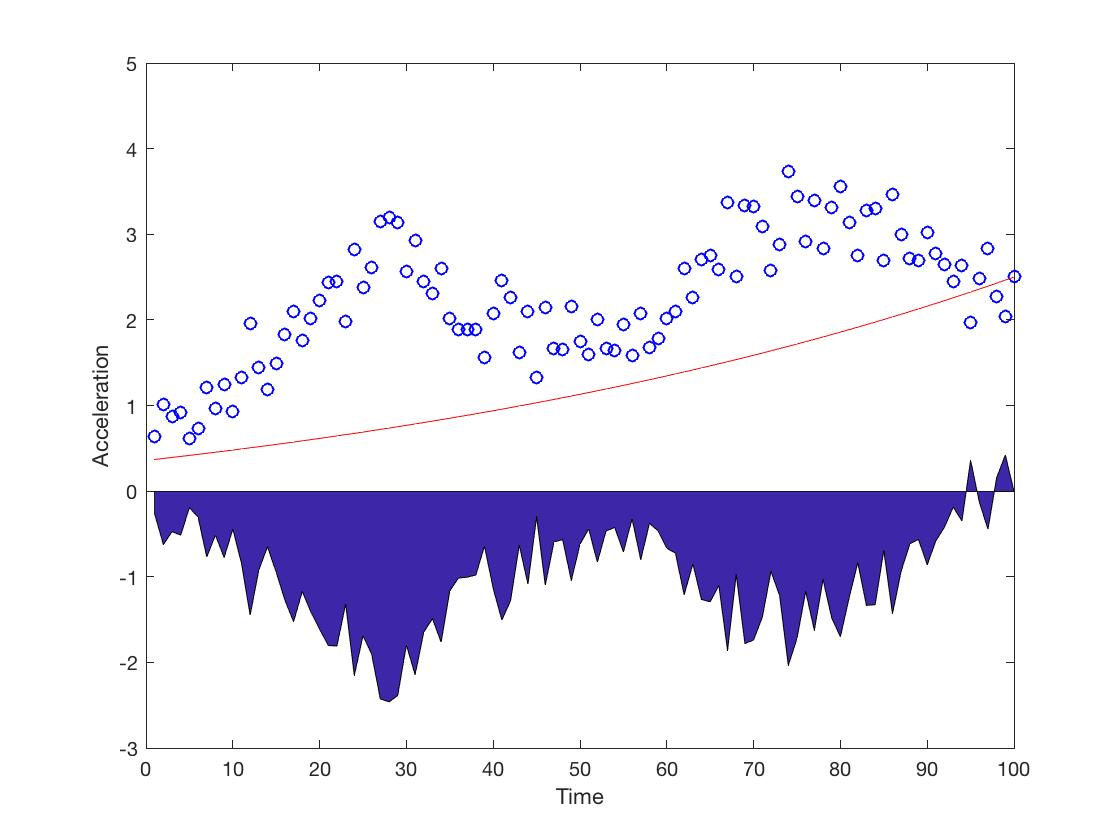
\includegraphics[width=\widthOfMatcherFigure]{figWR/matcher1}
\caption{Matcher Process, Wrong music}
\label{matcherStep0}
\end{figure}

\begin{figure}[H]
\centering
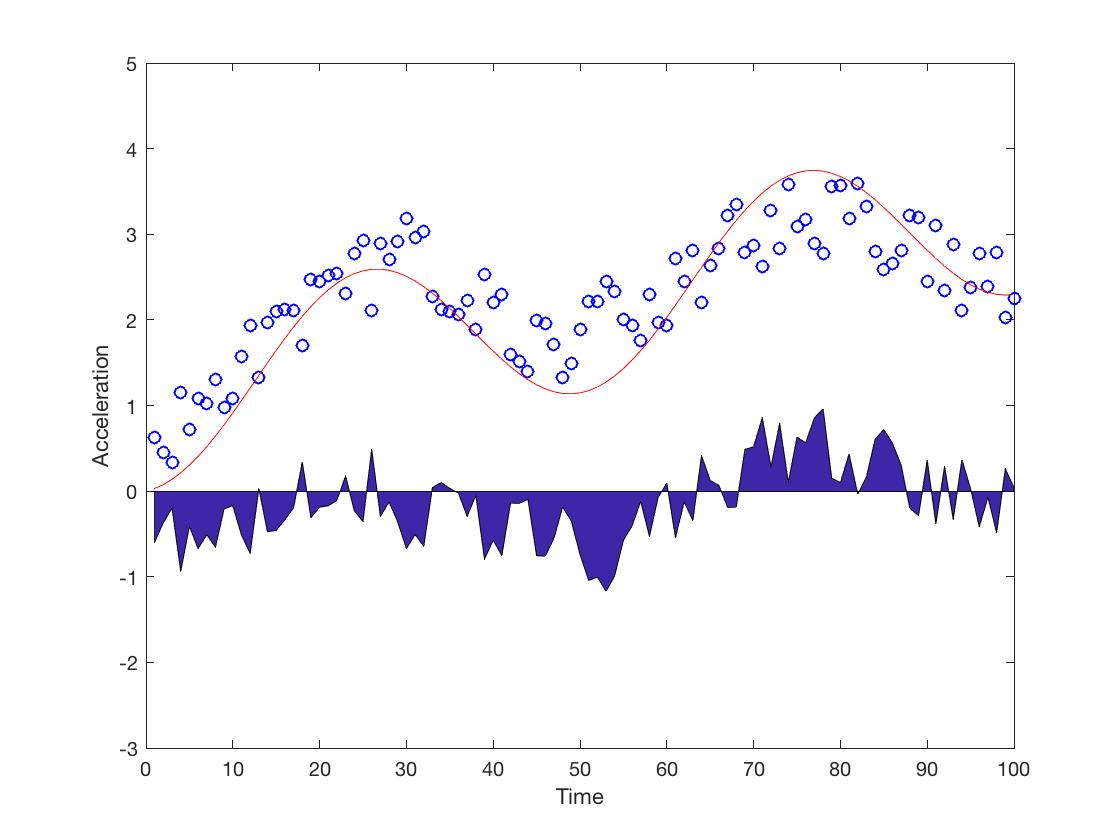
\includegraphics[width=\widthOfMatcherFigure]{figWR/matcher2}
\caption{Matcher Process, Right music}
\label{matcherStep1}
\end{figure}

\subsubsection{Mixer}

   After we have multiple sound tracks through either of the previous process,
   we mix them together and create the final audio. Feel free to play it.

\subsection{PC Terminal}

Besides the cellphone terminal part, we also designed a PC terminal part,
because when users dance, cellphones in hands are not safe enough. Cellphones
might be thrown out and hurt someone and then be broken. Moreover, the
cellphones are too heavy to carry when doing some fierce action. So developing a
safer and lighter bracelet is necessary. The second part of our product can
exactly satisfy the needs. 

The second part consists of a bracelet and a PC terminal. The bracelet contains
the sensor JY901, the bluetooth module and batteries. More specifically, the
sensor JY901 can detect data, the bluetooth module can transfer data to the
terminal and the batteries can power both JY901 and bluetooth. Overall, the
bracelet mainly does the detecting job. On the other hand, the PC terminal
mainly does the analyzing and generating jobs. The software on PC terminal
developed by Unity3D can apply several different algorithm to analyze the data,
so that the origin motion kind of the users can be defined. Then by comparing
different conditions prepared previously, the software can mix and play all
kinds audio source. 


\subsubsection{Hardware}
\paragraph{Attitude Sensor JY901}

The sensor JY901 is a attitude sensor that can detect the
acceleration, the angle of avertence and angular velocity. The sensor itself
consists of three-axis gyroscope, three-axis acceleration sensors, three-axis
digital compass and some other motion sensors. The sensor JY901 has the
following characteristics: 

\begin{itemize}
\item Flexible data outputting ports. (I2C, SPI, TTL are supported)
\item High speed data outputting rate. (Highest 500Hz)
\item Low power consumption. (17mA)
\item Short and stable initializing time. 
\item Support software development. 
\end{itemize}
\paragraph{Bluetooth Module}

It is connected with the JY901 sensor used for data transmission. In the serial
protocol, the bluetooth plays a role of an imaginary COM port whose name is
“COM6” on the Windows platform. 


\paragraph{Battery}

We use two chargeable batteries to power both JY901 sensor and the bluetooth
module. Each battery’s size is about 1cm*2cm*0.3cm which is very small. However,
each battery can provide 3.3V voltage and about 200 mAh electric charge. Since
the consumption of sensor JY901 is very small, the battery’s life is able to
ensure the normal work of our product. 


\paragraph{Fabrication}
\subsubsection{Software}
\paragraph{Data collection algorithm (same with the Mobile terminal part)}
\paragraph{Data transmission algorithm}

Programming Language: C\#

Input: All kinds of data collected by the sensor JY901, including acceleration,
angular acceleration, temperature and so on in 16 hexadecimal.   

 Output: Acceleration readings of three axises in 10 hexadecimal. 

 Algorithm: The algorithm includes mainly two functions which are''
 ``ReceiveData()'' and'' ``ReadData()'' and they each has their own thread. In
 the initialization part “void Update()” function, we create and open two
 threads one by one which can ensure that the data path is clear and efficient.

 Then in function ``ReceiveData()'', an empty string and a buffer byte are
 created to store and transport the data collected. Since the “55” in 16
 hexadecimal equals to “85” in 10 hexadecimal and all the data we need starts
 with “55” in 16 hexadecimal, the “if” sentences are applied. After all the
 suitable datas have been collected, we add the string to the queue created as a
 data pool using the order “queueDataPool.Enqueue(string)”. 

 In function ``ReadData()'', we first use the thread different from the previous
 one. All the data source in the part are from the queue acting as data pool.
 Here another buffer is created to store the data read out of the queue. We read
 data out one by one, when the length of the buffer reaches 22 which is the
 length we need, the buffer will be stored as formal data and then be cleared.
 Please note that since in the “ReceiveData” part we already judge what kind of
 data to collect, in the queue the data should starts with “85” in 10
 hexadecimal and we don’t need to set conditions again. Then there is the
 calculation part, take the data starts with “5551” in 16 hexadecimal as
 example. After “5551” the three axises accelerations are stored in two digits.
 The data format of the queue is “string”, so we need to transform data which is
 “string in 16 hexadecimal” to “int in 10 hexadecimal”. The function
 “Int16.Parse(stroutpool[4].ToString(),System.Globalization.NumberStyles.AllowHexSpecifier)” 
 is applied. Thus we can calculate the accelerations out one by one.  
\paragraph{Data analysis algorithm (same with the Mobile terminal part)}
\paragraph{Audio source generating algorithm (same with the Mobile terminal
  part)} 
\subsubsection{Working Principles}